


\documentclass[main]{subfiles}

\begin{document}


\chapter{Results}


This chapter includes the saliency metric and qualitative results gained from testing the method panel on ImageNet data and pre-trained CNN models. Insights on each method are summarised at the end of the chapter and compared with existing insights in the literature.

\section{Results Overview}

\subsection{Sample Sizes}  \label{sec:data_collection}
A set of 300 attributions for the full method panel took around 10 hours to collect and evaluate using a Nvidia GTX-1080 GPU. LIME was a key bottleneck due to its perturbation-based approach. After several hundred attributions the process also became very slow and would have to be restarted from that point (possibly due to a GPU memory leak in method internals). These performance considerations meant only 1000 instances out of 50,000 available in the validation set were used for evaluation. This was at least the same 1000 instances for all methods, and different dimensions were added to generate insights regardless: different attribution thresholds, and subsetting the results for high confidence (p $>0.9$) vs low confidence model predictions.

\subsection{Software Availability}

Code for the project is available on GitHub and is intended to be made public after improving the existing model agnosticity for practitioners as well as cleaning up dependencies and file structures. The framework has modular support for attribution methods provided they are compatible with image data and return an input-space representation of their explanation, and modular support for other saliency metrics as mentioned in Section \ref{sec:sw3}.


\subsection{Other Model Testing}

Some limitations were encountered on SHAP for ResNet50 and InceptionV3 architectures. Other methods were successfully tested on other models with results below, though the bug in SHAP was not resolved in time for project completion. The impact of this obstacle is discussed in the next chapter.

\section{Saliency Metric Results}
\subsection{VGG-16}

Figure \ref{vggAfig} shows IOU and IOU* statistics for a 1000-instance sample explaining VGG-16 model predictions. The 1000 instances are broken up into high confidence (top row) and low confidence predictions (bottom row), where high confidence refers to a model output of $p>0.9$. Error bars indicate one standard deviation from the mean result displayed by bar height, and can be used a proxy of method consistency. For this setup a threshold of 0.5 standard deviations was applied to the attribution output for IOU and 1 standard deviation for IOU*.\\

\vspace{0.2in}
Some observations on Figure \ref{vggAfig} (other observations in Section X):
\begin{itemize}
\item Results are similar for high vs low confidence predictions, with LIME's variance being one noticeable difference.
\item SHAP and DeepLift perform similarly on IOU but not IOU*
\item GradCAM scores lower on these metrics though is visually less noisy than DeepLIFT and SHAP
\end{itemize}


\newpage

%\vspace{2in}

\begin{figure}[h]\centering
\vfill
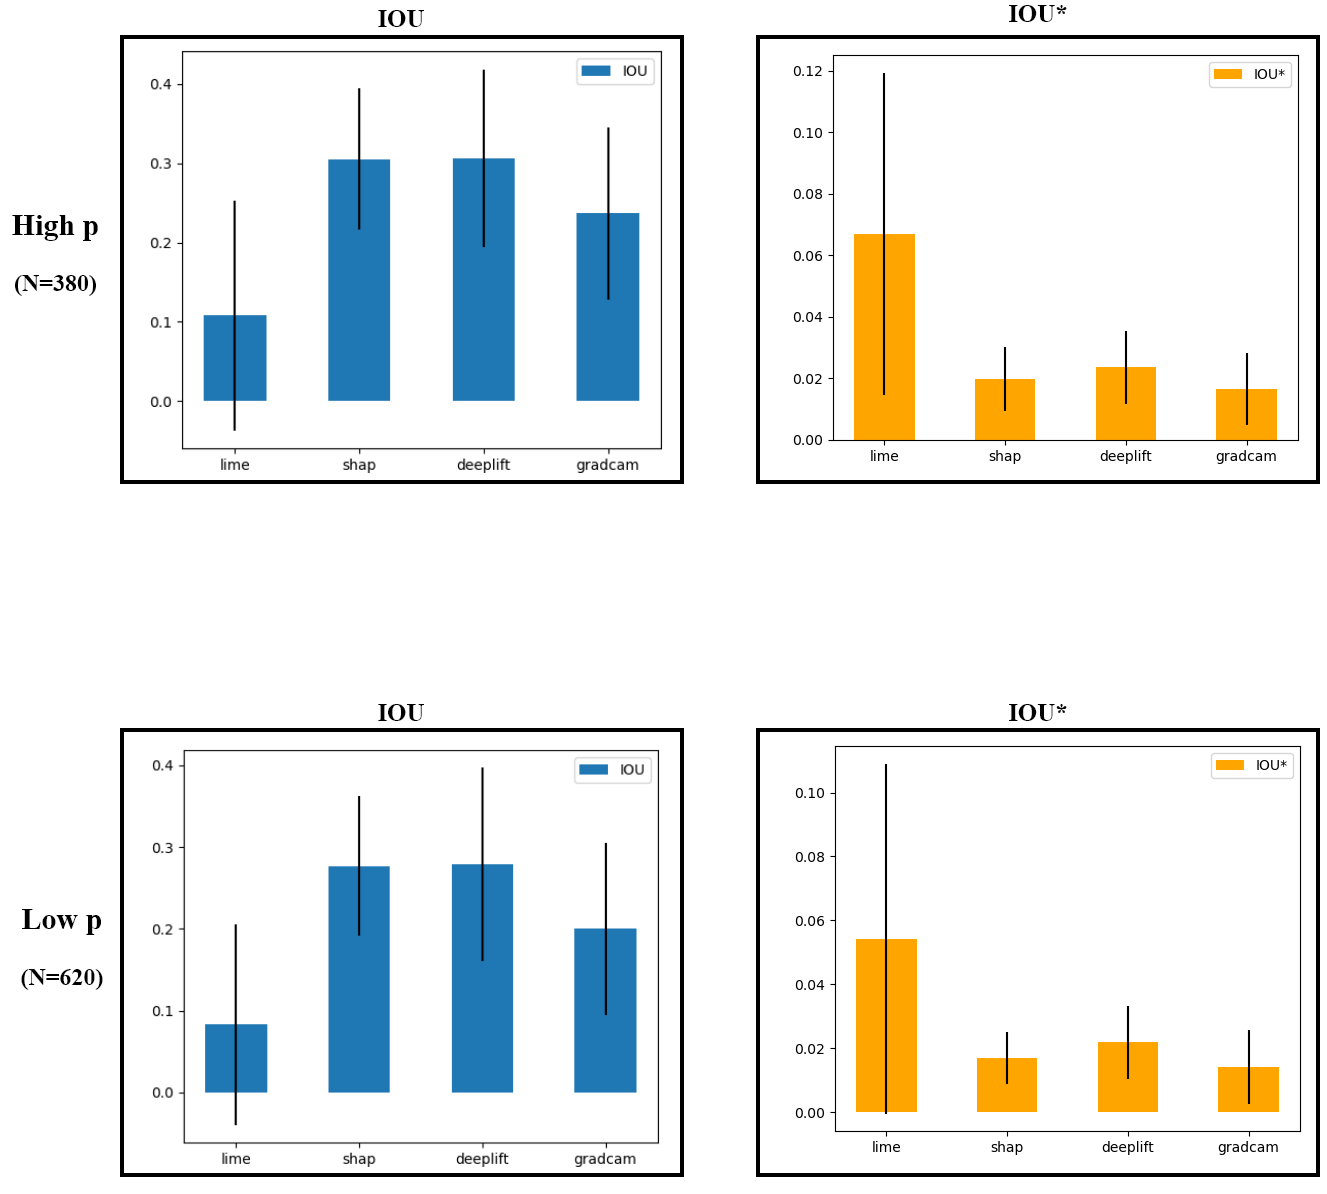
\includegraphics[scale=0.32]{vgg_0_5_and_1.png}
\caption{IOU, IOU* statistics for a 1000-instance attribution sample of VGG-16. }
\label{vggAfig}
\vfill
\end{figure}

In Appendix C, Figure X shows comparatively identical results for a smaller sample (N=300) with a different threshold set: 1 for IOU and 2 for IOU*.

\newpage



\subsection{InceptionV3}




\subsection{ResNet50}


\newpage
\section{Other Criteria}
\subsection{Method Performance}



\subsection{Consistency}
Refer to variances.

\subsection{Visual Observations}

\subsubsection{Localisation vs Pattern Discrimination}

\subsubsection{Impact of Thresholding}



\subsection{Compatibility \& Ideal Use Cases}

\subsubsection{SHAP}
\subsubsection{GradCAM}
\subsubsection{DeepLIFT}
\subsubsection{LIME}
%"While we have made a case for model agnosticism, this approach is not without its challenges. For example, getting a global understanding of the model may be hard if the model is very complex, due to the trade-off between flexibility and interpretability. To make matters worse, local explanations may be inconsistent with one another, since a flexible model may use a certain feature in different ways depending on the other features. In Ribeiro et al. (2016) we explained text models by selecting a small number of representative and non-redundant individual prediction explanations obtained via submodular optimization, similar in spirit to showing prototypes (Kim et al., 2014). However, it is unclear on how to extend this approach to domains such as images or tabular data, where the data itself is not sparse. In some domains, exact explanations may be required (e.g. for legal or ethical reasons), and using a black-box may be unacceptable (or even illegal). Interpretable models may also be more desirable when interpretability is much more important than accuracy, or when interpretable models trained on a small number of carefully engineered features are as accurate as black-box models."  Model-Agnostic Interpretability of Machine Learning

% mention low performance on oterh model archtiectures from Lit Review (ancona)




\section{Summary of Insights}
\subsection{Quantitative}

\subsection{Qualitative}


% LIME performance heavy num_samples parameter





Discuss developed software novelty



\end{document}